\documentclass[12pt,a4paper,fleqn, onesside]{report}
%
\usepackage[T1]{fontenc}
\usepackage{amsmath, amssymb, amsthm}
\usepackage[danish,english]{babel}

\usepackage[ansinew]{inputenc}
%\usepackage[utf8]{inputenc} %Der skal anvendes utf8
\usepackage{epsfig}
\usepackage{graphicx}
\usepackage[]{mcode}
\usepackage{lmodern}
\usepackage{float}
\usepackage{setspace}
\usepackage{lscape}
\usepackage{hyperref}
\usepackage{cleveref}
\crefname{equation}{}{equations}
\crefname{figure}{figure}{figures}
\usepackage{tabu}
\usepackage{graphicx}
\usepackage{caption}
\usepackage{multirow}
\usepackage{spverbatim}
\onehalfspacing

\usepackage[top=25mm, left=30mm, right=30mm,bottom=25mm,headsep=10mm, footskip=12mm]{geometry}
%
\usepackage{fancyhdr}
\pagestyle{fancyplain}
\lhead[\thepage]{}

\begin{document}

\begin{titlepage}
\begin{center}
\vspace{4cm}
\Huge{\sc 31310 Linear Control Design 2}\\
\vspace{0.8cm}
\large{\sc Compulsory Assignment 2015 : Loudspeaker control\\}
\vspace{1.2cm}
%\Huge {\sc Exam Report}\\
%\vspace{2cm}
\normalsize{by}\\
\vspace{1.2cm}
{\sc
\large Katleen Blanchet s150798  \\ 
Titouan Boulmier s150810\\
}
%\o{}
\vspace{2cm}
\begin{center}
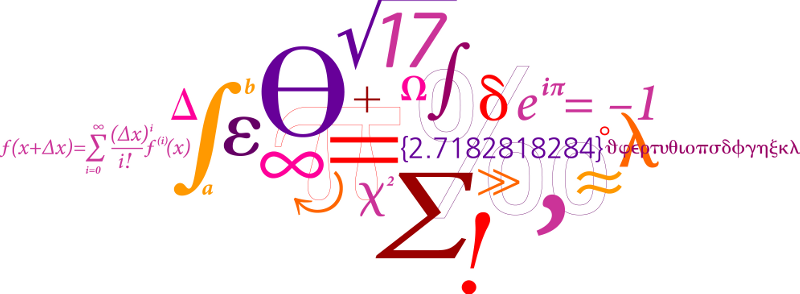
\includegraphics[scale=2.2]{dtulogo2.jpg}
\end{center} 
\vspace{3.1cm}
\normalsize{\today}\\
\vspace{1.37cm}
\includegraphics[scale=0.7]{dtulogo.jpg}\\
\vspace{0.2cm}
\normalsize{Technical University of Denmark \\ Department of Electrical Engineering \\
}
\end{center}
\end{titlepage}
%\newpage
\thispagestyle{empty}
\selectlanguage{english}

\pagebreak
\pagenumbering{Roman}
\setcounter{page}{1}
\setcounter{tocdepth}{4}
\setcounter{secnumdepth}{4} 
\tableofcontents
\newpage
\pagenumbering{arabic}
\def\chaptername{Exercice}


\chapter{Distortion Attenuation for Loudspeakers}
\section{Moving-coil Loudspeakers}
\subsection{Loudspeakers electrical equivalent circuit}

\begin{figure}[H]
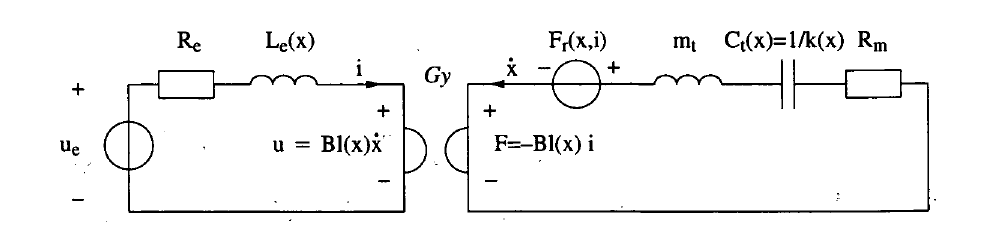
\includegraphics[scale=.6]{figures/circuit.png}
\caption{Electrical equivalent lumped element model of the voltage driven electrodynamic loudspeaker for low frequencies. The coupling between the electrical and mechanical domain is performed through the gyrator with gyration constant Bl(x).}
\label{circuit}
\end{figure}

\begin{align} 
  u_e &= R_ei+\frac{dL_e(x)}{dx}\frac{dx}{dt}i+L_e(x)\frac{di}{dt}+Bl(x)\frac{dx}{dt} \label{eq:1.1} \\     
  Bl(x)i &= m_t\frac{d^2x}{dt^2}+R_m\frac{dx}{dt}+k(x)x-\frac{1}{2}\frac{dL_e(e)}{dx}i^2 \label{eq:1.2}
\end{align}
where
\begin{align}
  Bl(x) &= Bl_0+b_1x+b_2x^2 \label{eq:1.3}  \\
  L_e(x) &= L_{e0}+l_1x+l_2x^2 \label{eq:1.4}  \\
  k(x) &= k_0+k_1x+k_2x^2 \label{eq:1.5} 
\end{align}

\subsection*{Problem 1}
\addcontentsline{toc}{subsubsection}{Problem 1}
By means of Eqs~\ref{eq:1.1},~\ref{eq:1.2},~\ref{eq:1.3},~\ref{eq:1.4} and~\ref{eq:1.5}, we can identify 3 state variables $x$,  $\dot{x}$ and $i$. We can also identify the input $u_e$.

$\text{x}=\begin{pmatrix}
   x \\
   \dot{x} \\
	 i
\end{pmatrix}$ and $\text{u}=(u_e)$

Then, we can derive the nonlinear dynamical state space model to obtain

\begin{align}
   \dot{x} &= \dot{x}\\
	 \ddot{x} &= \frac{(Bl_0+b_1x+b_2x^2)i-R_m\dot{x}-(k_0+k_1x+k_2x^2)x+\frac{1}{2}(l_1+2l_2x)\dot{x}i^2}{m_t}\\
	 \dot{i} &= \frac{u_e-(R_e+(l_1+2l_2x)\dot{x}^2)i-(Bl_0+b_1x+b_2x^2)\dot{x}}{L_{e0}+l_1x+l_2x^2}
\end{align}

In matrix format, we have

\begin{equation}
	\label{eq:eqModel}
	\dot{\text{x}}=f(\text{x})+g(\text{x})\text{u}
\end{equation}
with
\begin{equation}
	\label{eq:f(x)}
	f(\text{x})=\begin{pmatrix}
   \text{x}(2) \\
	 \frac{(Bl_0+b_1\text{x}(1)+b_2\text{x}(1)^2)\text{x}(3)-R_m\text{x}(2)-(k_0+k_1\text{x}(1)+k_2\text{x}(1)^2)\text{x}(1)+\frac{1}{2}(l_1+2l_2\text{x}(1))\text{x}(2)\text{x}(3)^2}{m_t}\\
	 \frac{-(R_e+(l_1+2l_2\text{x}(1))\text{x}(2)^2)\text{x}(3)-(Bl_0+b_1\text{x}(1)+b_2\text{x}(1)^2)\text{x}(2)}{L_{e0}+l_1\text{x}(1)+l_2\text{x}(1)^2}
\end{pmatrix}
\end{equation}
\begin{equation}
	\label{eq:g(u)}
	g(\text{x})=\begin{pmatrix}
   0\\
   0 \\
	 1
\end{pmatrix}
\end{equation}

\subsection*{Problem 2}
\addcontentsline{toc}{subsubsection}{Problem 2}
The block diagram of the nonlinear model figure \ref{fig:figP2} in Appendix \ref{AppP2} shows how the electrical and the mechanical subsystems are interconnected. This block diagram is also our SIMULINK model. The system is quickly stabilised (around 1 s) but as we are going to analyse it in the frequency domain, a longer period of time will provide better results. Thus, the TIME\_SIM is set to 5 s. 

\subsection*{Problem 3}
\addcontentsline{toc}{subsubsection}{Problem 3}
The input voltage is set to $u_e = A_u sin(2\pi f_c t)$, where $A_u = 5 \ V$ and $f_c = 20 \ Hz$.
Then the nonlinear system implemented in P2 is simulated to get the states responses. For more clarity, the time domain responses were plotted from 0 to 2s. Moreover, the system is not stabilised at the beginning of the simulation, so it was decided to remove the first second for the spectral analysis. To visualise the signals in the frequency domain, we used the \textit{$power\_spectral\_density$} function given in the assignment \cite{assign} with $F_s = \frac{1}{TIME\_SIM} = 10 \ kHz$. The function output gives the power spectral density $P_{xx}$ in [$Amplitude^2$/Hz]. In order to convert it in [dB/Hz], we use: 
\begin{equation*}
P_{dB} = 10log_{10}(P_{xx})
\end{equation*} 

\begin{figure}[H]
 \centering 
 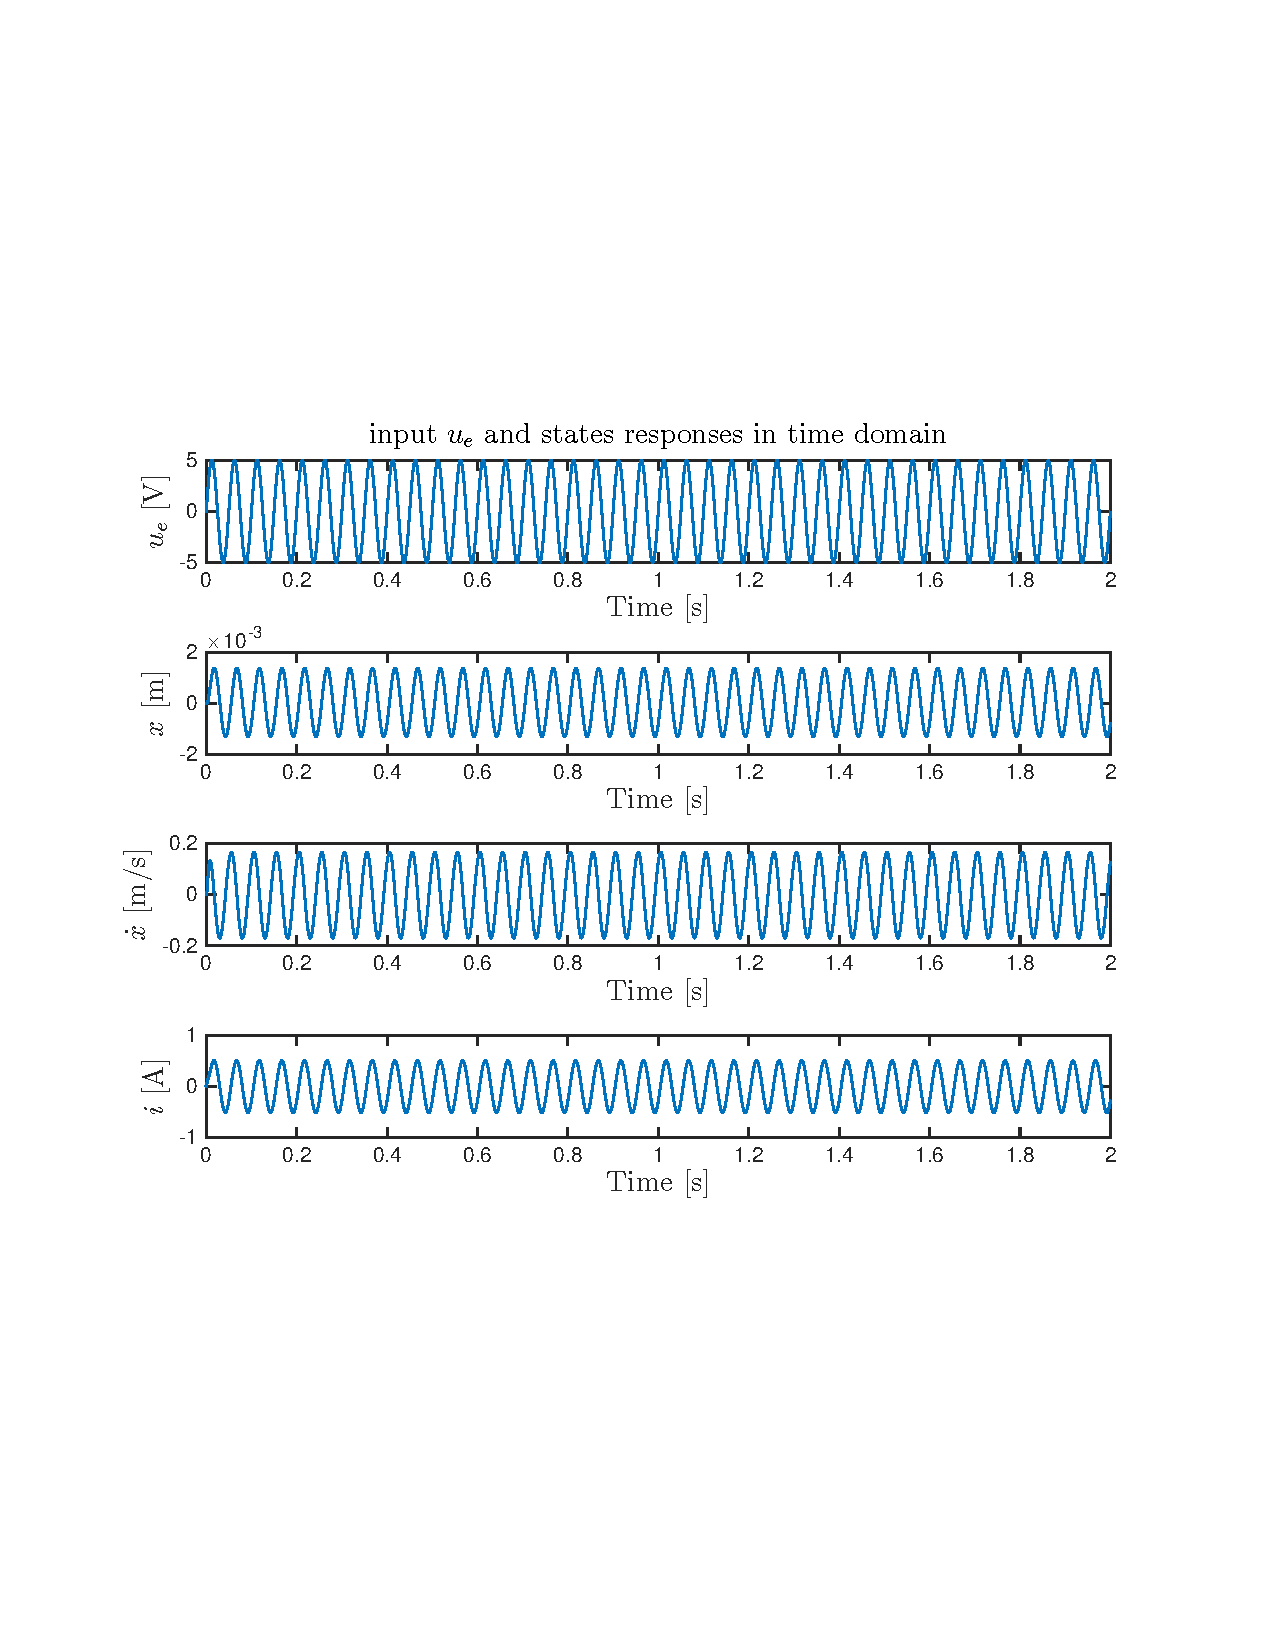
\includegraphics[trim=2cm 7cm 2cm 7cm, clip=true, totalheight=0.35\textheight, angle=0]{figures/P3timeDomain.pdf}
 \caption{Nonlinear Model: input $u_e$ and the states responses in the time domain}
 \label{fig:NLMt}
\end{figure}

\begin{figure}[H]
 \centering 
 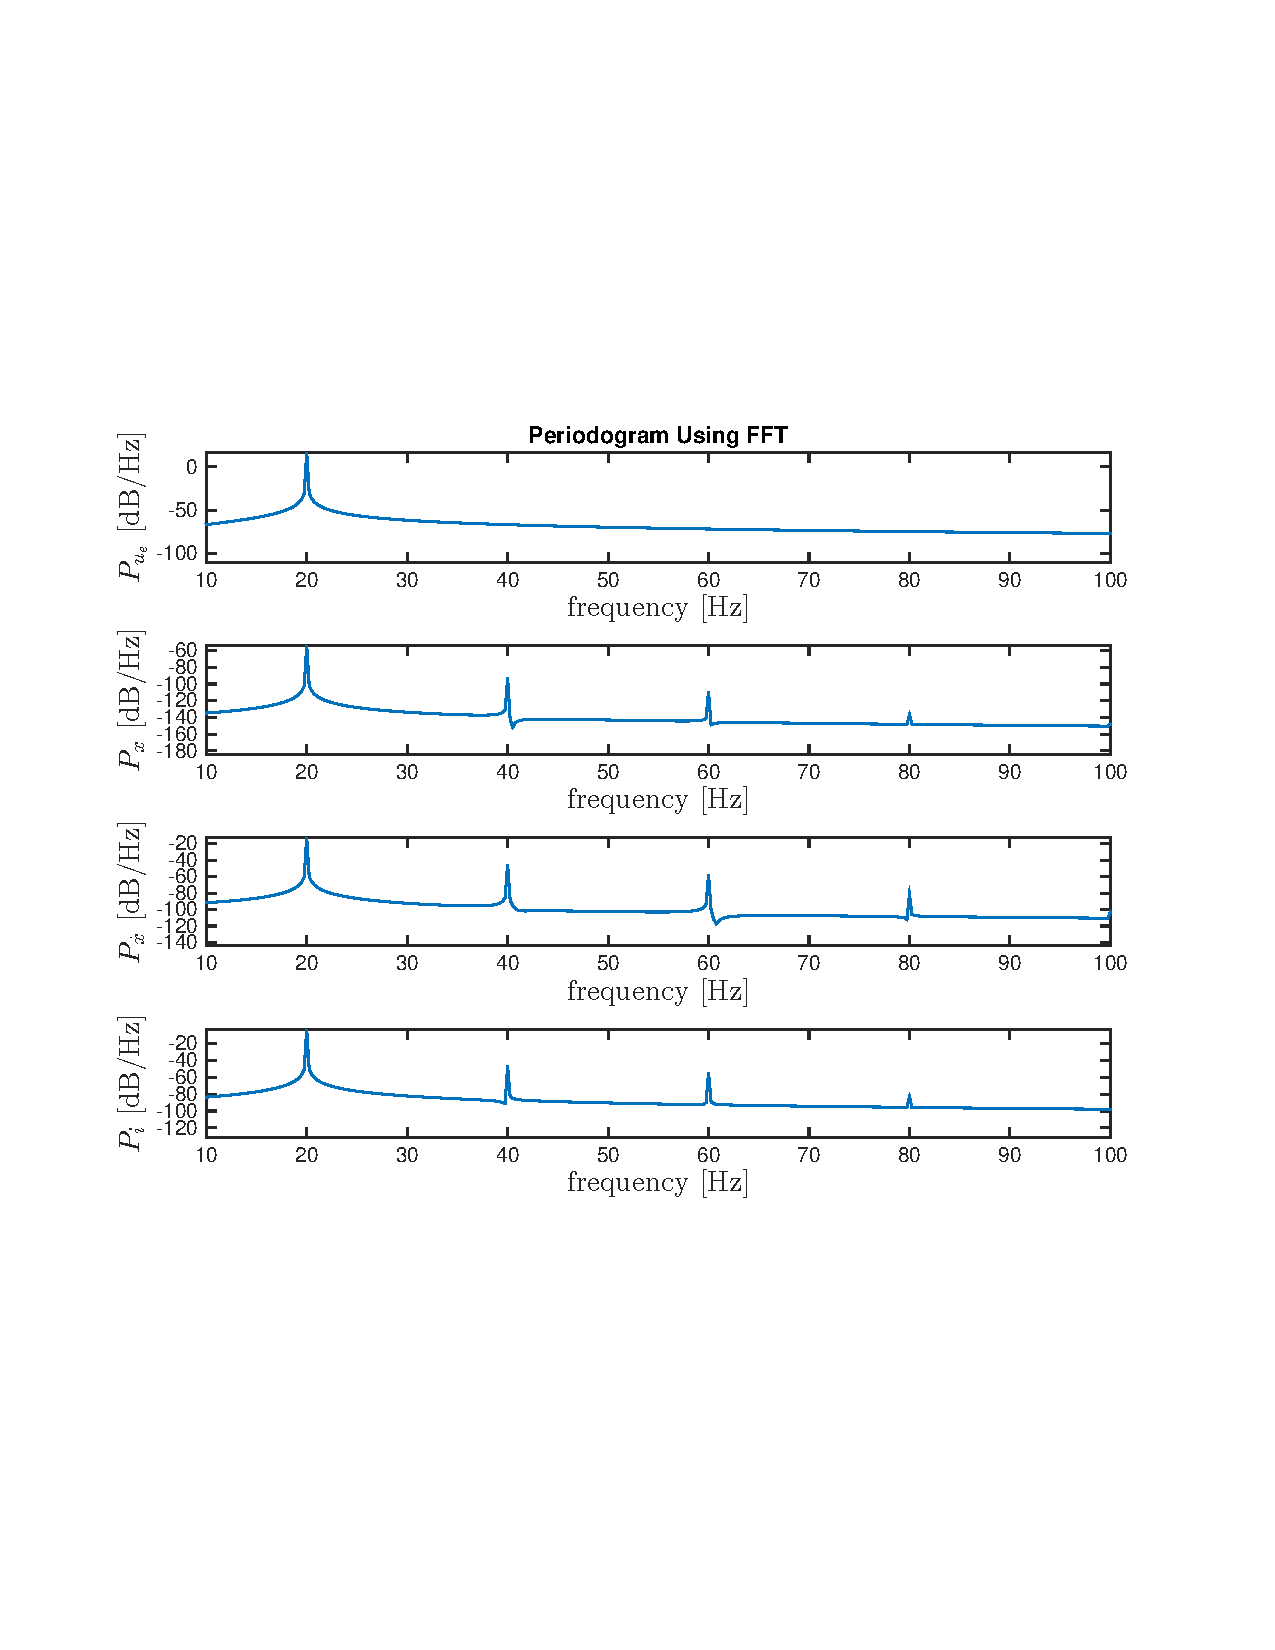
\includegraphics[trim=2cm 7cm 2cm 7cm, clip=true, totalheight=0.35\textheight, angle=0]{figures/P3frequencyDomain.pdf}
 \caption{Nonlinear Model: input $u_e$ and the states responses in the frequency domain}
 \label{fig:NLMf}
\end{figure}

In the time domain (see figure \ref{fig:NLMt}), we notice that the states responses are sinusoidal, with constant amplitudes. The system looks stable. Moreover, the frequency of the states seems similar to the frequency of the input signal, with slight variations. The explanation for these changes is given in the frequency domain, figure \ref{fig:NLMf}, where we can see several more spikes at the frequencies $f_n = nf_c$, smaller than the fundamental one at $f_c = 20 \ Hz$. The presence of other harmonics in the states responses, which are not in the input, shows the effects of the nonlinearity of the system. It may due to the fact that the voice coil displacement is limited: when it goes too far, the spider prevents it from leaving the magnetic field, which can cause the harmonic distortion. 

\subsection{Harmonic Distortion}
We are now going to study the harmonic distortion observed in the states responses in the frequency domain. 
\subsection*{Problem 4}
\addcontentsline{toc}{subsubsection}{Problem 4}
The analysis will be restricted to the voice coil velocity $\dot{x}$. The Total Harmonic Distortion (THD) is described by
\begin{equation}
THD = \frac{\sqrt{\sum_{n=2}^{N}A_n^2}}{\sqrt{\sum_{n=1}^{N}A_n^2}} \ 100\%
\end{equation}
where $A_1$ the amplitude of the fundamental frequency and $A_n$ the amplitudes of the harmonics. 

To compute THD for the 5 harmonics after the fundamental frequency $f_c$ we need to find the 6 amplitudes corresponding to the fundamental frequency pikes and the 5 following harmonics. To that purpose, a function \textit{amplitude} was implemented (see below) with \textit{\text{x}} the signal and \textit{fr} the frequency at which we desire to know the amplitude of the spike. The Fast Fourier Transform is computed but not the spectral power density as previously. 
\begin{lstlisting}[language=Matlab]
function [ res ] = amplitude(x, TIME_SIM, fr)
	NFFT = length(x);
	X = fft(x,NFFT)/(NFFT);	
	X = 2*abs(X(1:NFFT/2+1)); 
	res = X(fr*TIME_SIM+1);
end
\end{lstlisting}

Finally for a TIME\_SIM = 5s, for the voice coil velocity $THD = 2.57 \ \%$. 
We then use the equations \eqref{d2} and \eqref{d3} to compute the second and third order harmonic distortion. We obtain $d_2 = 2.48 \ \%$ and $d_3 = 0.65 \ \%$.
\begin{equation}
d_2 = \frac{A_2}{\sqrt{A_1^2 + A_2^2}} \ 100\%
\label{d2}
\end{equation}
\begin{equation}
d_3 = \frac{A_3}{\sqrt{A_1^2 + A_3^2}} \ 100\%
\label{d3}
\end{equation}

We can notice that $d_2$ corresponds to the THD calculated for $N=2$. Because the amplitudes of the harmonics decrease when the order gets bigger, it is logical that the values of THD and $d_2$ are quite similar. On the contrary, $A_3$ is negligible in front of $A_1$, that why $d_3$ is small and far from the THD. 
\subsection*{Problem 5}
\addcontentsline{toc}{subsubsection}{Problem 5}
In order to study the effect of the variations of the frequency $f_c$ and the amplitude $A_u$ of the input $u_e$ on the second and third order harmonic distortion, we have computed $d_2$ and $d_3$ for a range of $A_u$ and $f_c$. The results can be seen on the figure \ref{fig:d2d3}. According to the graphic, the variations of the amplitude of the input do not affect the shape of the distortion levels. The amplitude has only an impact on the value of the distortion from 20 to 60 Hz. If it doubles, the pourcentage of the distortion will also be multiplied by two. On the other hand, when the fundamental frequency increases, the distortion levels $d_2$ and $d_3$ are stabilising at low values, nearly 0\% for $d_3$. It can be explained by the fact that the more the fundamental frequency grows, the more the harmonic pikes will be far from it as they correspond to $nf_c$. Their amplitude will be affected and will become of minor importance in front of the amplitude of the fundamental pike.

\begin{figure}[H]
 \centering 
 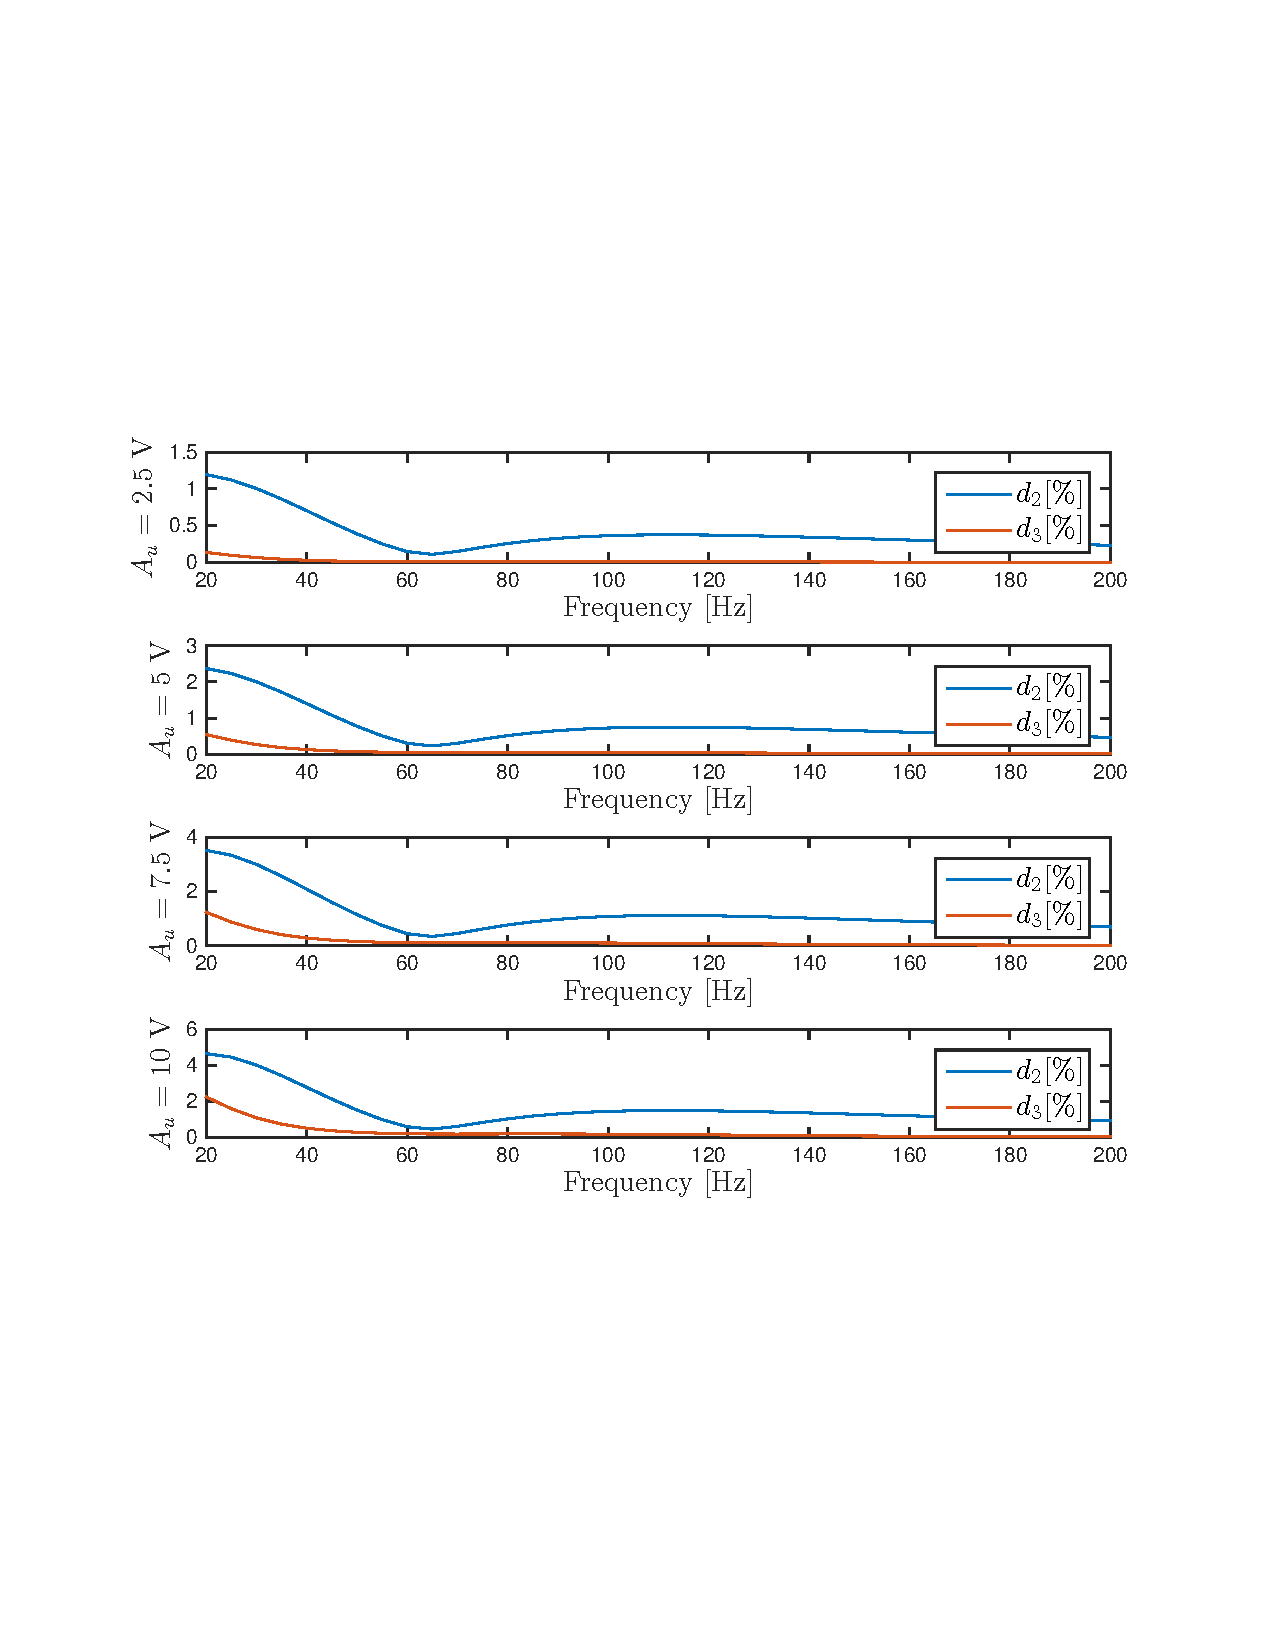
\includegraphics[trim=2cm 7cm 2cm 7cm, clip=true, totalheight=0.35\textheight, angle=0]{figures/P5d2d3.pdf}
 \caption{Effect of the variations of the frequency $f_c$ and the amplitude $A_u$ of the input $u_e$ on the second and third order harmonic distortion}
 \label{fig:d2d3}
\end{figure}

\subsection{Linearised Model}
The measured output is set to the voice coil current. Therefore $y(t) = i(t)$.
We also take $u_{e} = 0$ for the analysis of the linear and nonlinear model around the resting position of the voice coil. 

\subsection*{Problem 6}
\addcontentsline{toc}{subsubsection}{Problem 6}
All time derivatives are set to zero in order to determine the stationary states. Therefore, we have $\frac{dx}{dt} = 0$ and equations \eqref{eq:1.1} and \eqref{eq:1.2} are rewritten below:
\begin{align}
   u_{e} &= R_{e}i \label{stateq1} \\
   Bl(x)i &= k(x)x \label{stateq2}
\end{align}

As $u_{e} = 0$, from \eqref{stateq1} we obtain $i = 0$ and we deduce by substituting in \eqref{stateq2} that $k(x)x = 0$. Then $k(x) = 0$ or $x = 0$. The discriminant of the polynomial $k(x)$ of degree 2 is $\Delta = k_{1}^2-4k_{2}k_{0} < 0$. The voice coil displacement $x$ being real, we discard this value and get:
\begin{equation*}
\text{x}_{0}=
\begin{pmatrix}
  0 \\
  0 \\
  0
\end{pmatrix}
\end{equation*}

We linearise the model $\dot{\text{x}} = h(\text{x},\text{u})$ with $h(\text{x}) = f(\text{x}) + g(\text{x})\text{u}$ around the stationary states:
\begin{align*}
   x(t) &= x_{0} + \Delta x(t) = \Delta x(t)\\
   \dot{x}(t) &= \dot{x}_{0} + \Delta \dot{x}(t) = \Delta \dot{x}(t) \\
   i(t) &= i_{0} + \Delta i(t) = \Delta i(t)
\end{align*}

The linear model can then be written in the form:
\begin{align*}
   \dot{\text{x}} &= A\text{x} + B\text{u} \\
   y &= C\text{x}
\end{align*}

where \begin{equation*} A = \begin{pmatrix}
  \frac{\partial{h_{1}}}{\partial{\text{x}_{1}}} & \frac{\partial{h_{1}}}{\partial{\text{x}_{2}}} & \frac{\partial{h_{1}}}{\partial{\text{x}_{3}}} \\
  \frac{\partial{h_{2}}}{\partial{\text{x}_{1}}} & \frac{\partial{h_{2}}}{\partial{\text{x}_{2}}} & \frac{\partial{h_{2}}}{\partial{\text{x}_{3}}} \\
  \frac{\partial{h_{3}}}{\partial{\text{x}_{1}}} & \frac{\partial{h_{3}}}{\partial{\text{x}_{2}}} & \frac{\partial{h_{3}}}{\partial{\text{x}_{3}}}
\end{pmatrix}_{\text{x}_{0}}
\qquad B = \begin{pmatrix}
\frac{\partial{h_{1}}}{\partial{\text{u}}} \\
\frac{\partial{h_{2}}}{\partial{\text{u}}} \\
\frac{\partial{h_{3}}}{\partial{\text{u}}}
\end{pmatrix}_{\text{x}_{0}}
\qquad C = \begin{pmatrix}
\frac{\partial{r}}{\partial{\text{x}_{1}}} & \frac{\partial{r}}{\partial{\text{x}_{2}}} & \frac{\partial{r}}{\partial{\text{x}_{3}}} 
\end{pmatrix}_{\text{x}_{0}}
\end{equation*}

We obtain:
\begin{equation*} 
\frac{\partial{h_{1}}}{\partial{\text{x}_{1}}} = 0 \qquad \frac{\partial{h_{1}}}{\partial{\text{x}_{2}}} = 1 \qquad \frac{\partial{h_{1}}}{\partial{\text{x}_{3}}} = 0
\end{equation*}
\begin{equation*}
\frac{\partial{h_{2}}}{\partial{\text{x}_{1}}} = \frac{b_{1}\text{x}_{30} + 2b_{2}\text{x}_{10}\text{x}_{30} - (k_{0}+2k_{1}\text{x}_{10}+3k_{2}\text{x}_{10}^2) + l_{2}\text{x}_{20}\text{x}_{30}^2}{m_{t}}
\end{equation*}
\begin{equation*}
\frac{\partial{h_{2}}}{\partial{\text{x}_{2}}} = \frac{-R_{m} + \frac{1}{2}\times (l_{1}+2l_{2}\text{x}_{10})\text{x}_{30}^2}{m_{t}}
\end{equation*}
\begin{equation*}
\frac{\partial{h_{2}}}{\partial{\text{x}_{3}}} = \frac{Bl_{0}+b_{1}\text{x}_{10}+b_{2}\text{x}_{10}^2+(l_{1}+2l_{2}\text{x}_{10})\text{x}_{20}\text{x}_{30}}{m_{t}}
\end{equation*}
\begin{multline*}
\frac{\partial{h_{3}}}{\partial{\text{x}_{1}}} = \frac{(-2l_{2}\text{x}_{20}^2\text{x}_{30}-(b_{1}+2b_{2}\text{x}_{10})\text{x}_{20}) \times (L_{e0}+l_1\text{x}_{10}+l_2\text{x}_{10}^2)}{(L_{e0}+l_1\text{x}_{10}+l_2\text{x}_{10}^2)^2} - (l_{1}+2l_{2}\text{x}_{10}) \times \\
\frac{(-(R_e+(l_1+2l_2\text{x}_{10})\text{x}_{20}^2)\text{x}_{30}-(Bl_0+b_1\text{x}_{10}+b_2\text{x}_{10}^2)\text{x}_{20})}{(L_{e0}+l_1\text{x}_{10}+l_2\text{x}_{10}^2)^2}
\end{multline*}
\begin{equation*}
\frac{\partial{h_{3}}}{\partial{\text{x}_{2}}} = - \frac{2(l_1+2l_2\text{x}_{10})\text{x}_{20}\text{x}_{30}+Bl_0+b_1\text{x}_{10}+b_2\text{x}_{10}^2}{L_{e0}+l_1\text{x}_{10}+l_2\text{x}_{10}^2}
\end{equation*}
\begin{equation*}
\frac{\partial{h_{3}}}{\partial{\text{x}_{3}}} = - \frac{(l_1+2l_2\text{x}_{10})\text{x}_{20}^2+R_{e}}{L_{e0}+l_1\text{x}_{10}+l_2\text{x}_{10}^2}
\end{equation*}
\begin{equation*}
\frac{\partial{h_{1}}}{\partial{\text{u}}} = 0 \qquad 
\frac{\partial{h_{2}}}{\partial{\text{u}}} = 0 \qquad
\frac{\partial{h_{3}}}{\partial{\text{u}}} = \frac{1}{L_{e0}+l_1\text{x}_{10}+l_2\text{x}_{10}^2}
\end{equation*}
\begin{equation*}
\frac{\partial{r}}{\partial{\text{x}_{1}}} = 0 \qquad 
\frac{\partial{r}}{\partial{\text{x}_{2}}} = 0 \qquad
\frac{\partial{r}}{\partial{\text{x}_{3}}} = 1
\end{equation*}\\
We then substitute $\text{x}_{10} = \text{x}_{20} = \text{x}_{30} = 0$.
Finally, we get:
\begin{equation*} A = \begin{pmatrix}
   0 & 1 & 0 \\
   -\frac{k_0}{m_t} & -\frac{R_m}{m_t} & \frac{Bl_0}{m_t} \\
  0 & - \frac{Bl_0}{L_{e0}} & - \frac{R_e}{L_{e0}}  
\end{pmatrix}
\qquad B = \begin{pmatrix}
0 \\
0 \\
\frac{1}{L_{e0}}
\end{pmatrix}
\qquad C = \begin{pmatrix}
	0 & 0 & 1 
\end{pmatrix}
\end{equation*}\\
Numerically
\begin{equation} A = \begin{pmatrix}
   0 & 1 & 0 \\
  -1.20 \cdot 10^5 & -50.46 & 279.19 \\
  0 & -2.57 \cdot 10^3 & -1.40 \cdot 10^3
\end{pmatrix}
\qquad B = \begin{pmatrix}
0 \\
0 \\
177
\end{pmatrix}
\qquad C = \begin{pmatrix}
	0 & 0 & 1 
\end{pmatrix}
\label{eq:AandB}
\end{equation}\\
We can check these results with the matlab function \textit{linmod(model,$\text{x}_0$,$u_e$)}:
\vspace*{-0.5cm}
\begin{lstlisting}[language=Matlab]
[A,B,C,D] = linmod('nonLinearModel',[0;0;0],0);
\end{lstlisting}

\subsection*{Problem 7}
\addcontentsline{toc}{subsubsection}{Problem 7}
In this problem, we draw the block diagram of the linearised loudspeaker (see figure \ref{fig:linearModel} in Appendix \ref{AppLinearModelP7}) showing the couplings between the different states.

By means of this block diagram, we can make preliminary assessments of the system. Indeed, we can see that the state $i$ seems to be controllable and observable as it is connected to the input $u_e$ and to the output. However, the states $x$ and $\dot{x}$ seem to be controllable as they are also connected to the input $u_e$ but not observable because they are not connected to any output. Moreover the 3 states seem to be stable because of the 2 back-loops.

We can verify our assumptions regarding the controllability and the observability by calculating the $rank$ of $M_c$ and $M_o$.
\begin{lstlisting}[language=Matlab]
Mc = [B A*B A^2*B];
rank(Mc) % = 3 controllable
Mo=[C
    C*A
    C*A^2];
rank(Mo) % = 3 observable
\end{lstlisting}




\subsection*{Problem 8}
\addcontentsline{toc}{subsubsection}{Problem 8}
We can derive analytically the eigenvalues of the system dynamical matrix $A$.

\begin{align}
	\label{eq:eigenValues}
	det(\lambda I-A) & =det\begin{pmatrix}
 \lambda & -1 & 0 \\
  \frac{k_0}{m_t} & \lambda+\frac{R_m}{m_t} & -\frac{Bl_0}{m_t} \\
  0 & \frac{Bl_0}{Le_0} & \lambda+\frac{Re}{Le_0}
\end{pmatrix} \\
& = \lambda^3 +\left(\frac{Re}{Le_0}+\frac{Rm}{m_t}\right)\lambda^2+\left(\frac{RmRe+Bl_0}{m_tLe_0}+\frac{k_0}{m_t}\right)\lambda+\frac{k_0Re}{m_tLe_0}
\end{align}

We therefore have a third-order polynomial which can be solved with MATLAB but the eigenvalues can also be calculated using
\begin{lstlisting}[language=Matlab]
lambda = eig(A);
\end{lstlisting}

Thus, we obtain
\begin{equation}
	\label{eq:eigenValuesValues}
	\lambda = 1,0.10^2\begin{pmatrix}
	-2.9573 \\
	-5.7648 + 4.8571i\\
	-5.7648 - 4.8571i
	\end{pmatrix}
\end{equation}

We can notice that
\begin{equation}
	\label{eq:eigenValuesRe}
	Re(\lambda_i)<0, \ i=1,2,3
\end{equation}

which means that the system is asymptotically stable. Moreover, the eigenmodes of the system are $e^{\lambda_1t}$, $e^{\lambda_2t}$ and $e^{\lambda_3t}$. We can notice that \begin{equation*}
\frac{1}{\lambda_1}=\tau_1>\tau_2, \tau_3
\end{equation*}
which means that the response of the state $x$ to an input $u_e$ will be slower than the one of $i$ and $\dot{x}$. We can also see that as $\lambda_2$ and $\lambda_3$ have an imaginary part which means that $\dot{x}$ and $i$ will have an oscillatory response.


\subsection*{Problem 9}
\addcontentsline{toc}{subsubsection}{Problem 9}
Using the results of Problem 6 (\ref{eq:AandB}), we can implement a SIMULINK model (see figure \ref{fig:linearModelMatrix} in Appendix \ref{AppLinearModelP9}) of the linear system.

Then, we can simulate the linearised model with an input $u_e=A_u\sin(2\pi f_ct)$, where $A_u=5V$ and $f_c=20Hz$. The states response in the time domain is plotted figure \ref{fig:responseLMt} and the PSD is plotted figure \ref{fig:responseLMf}.

\begin{figure}[H]
 \centering 
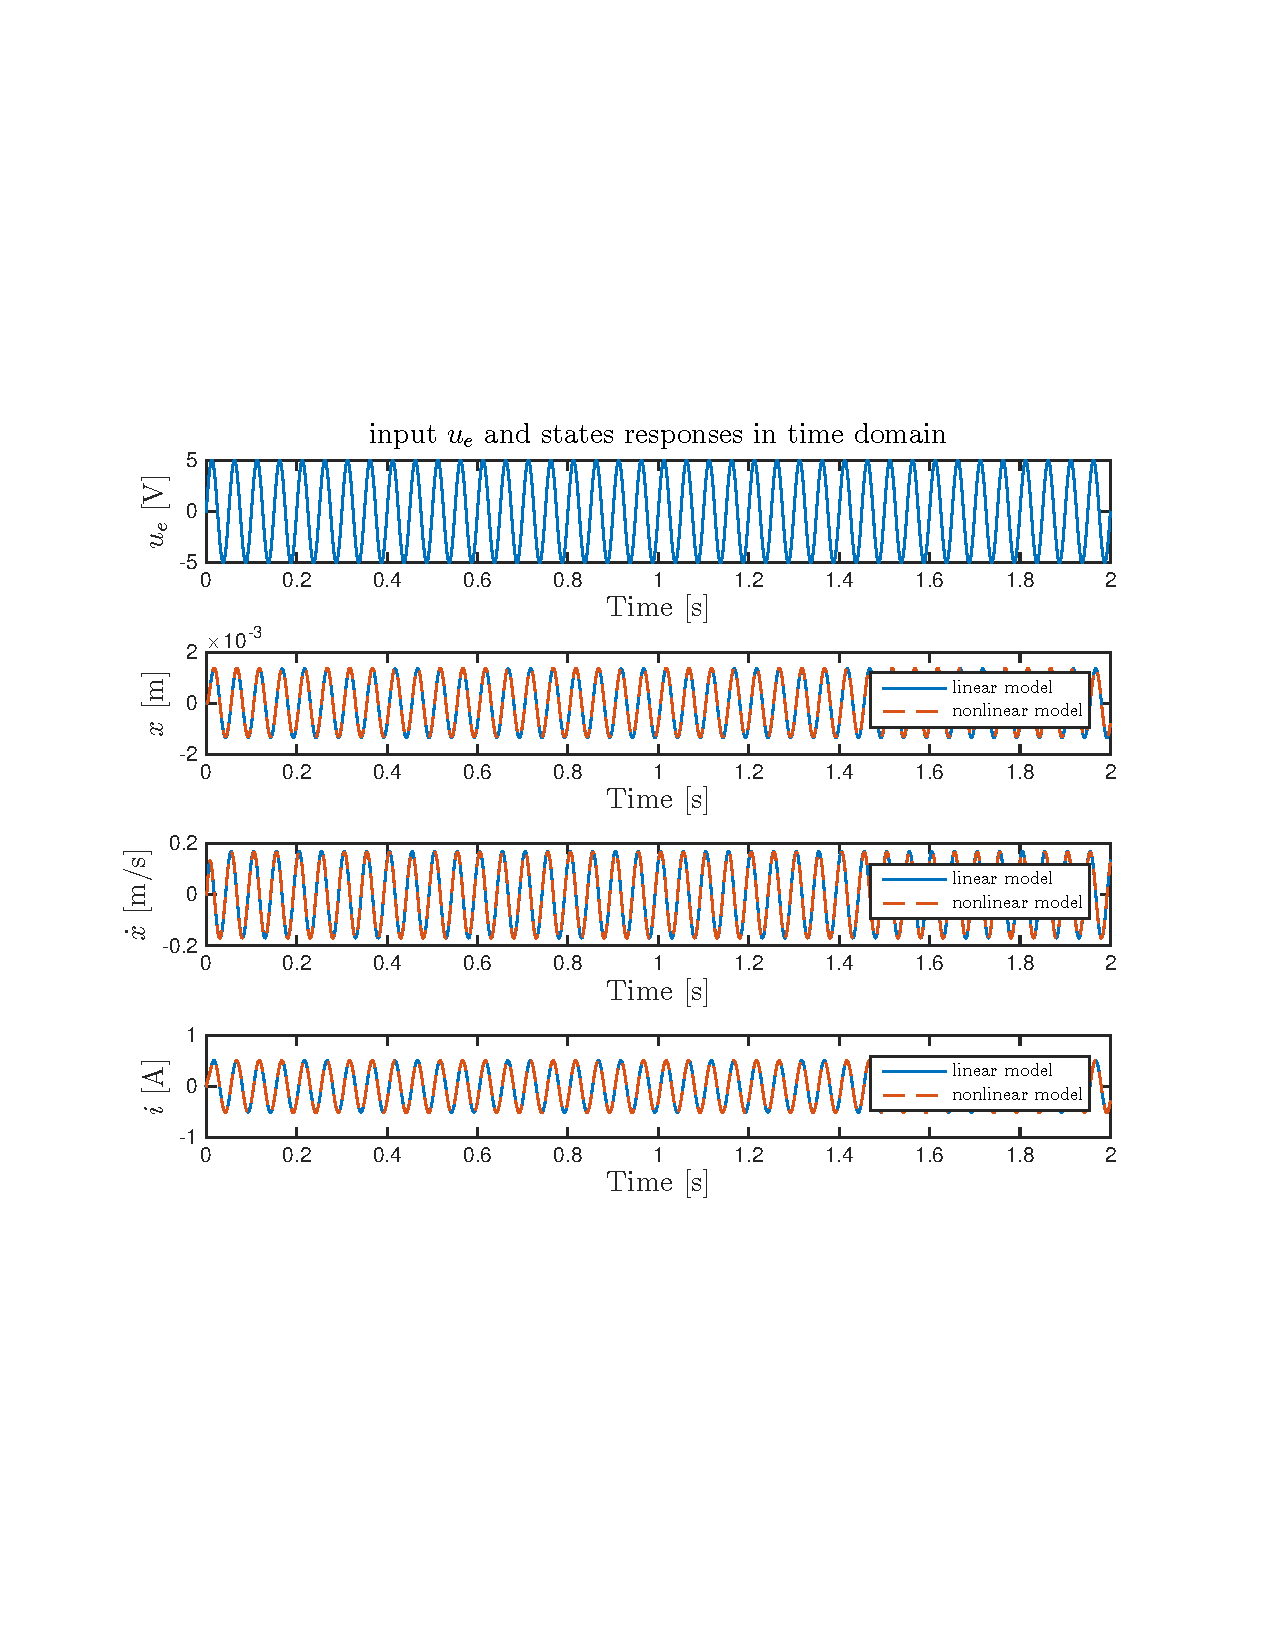
\includegraphics[trim=2cm 7cm 2cm 7cm, clip=true, totalheight=0.35\textheight, angle=0]{figures/p9time.pdf}
\caption{$u_e$ and states reponse to $u_e$ in time domain}
\label{fig:responseLMt}
\end{figure}
\begin{figure}[H]
 \centering 
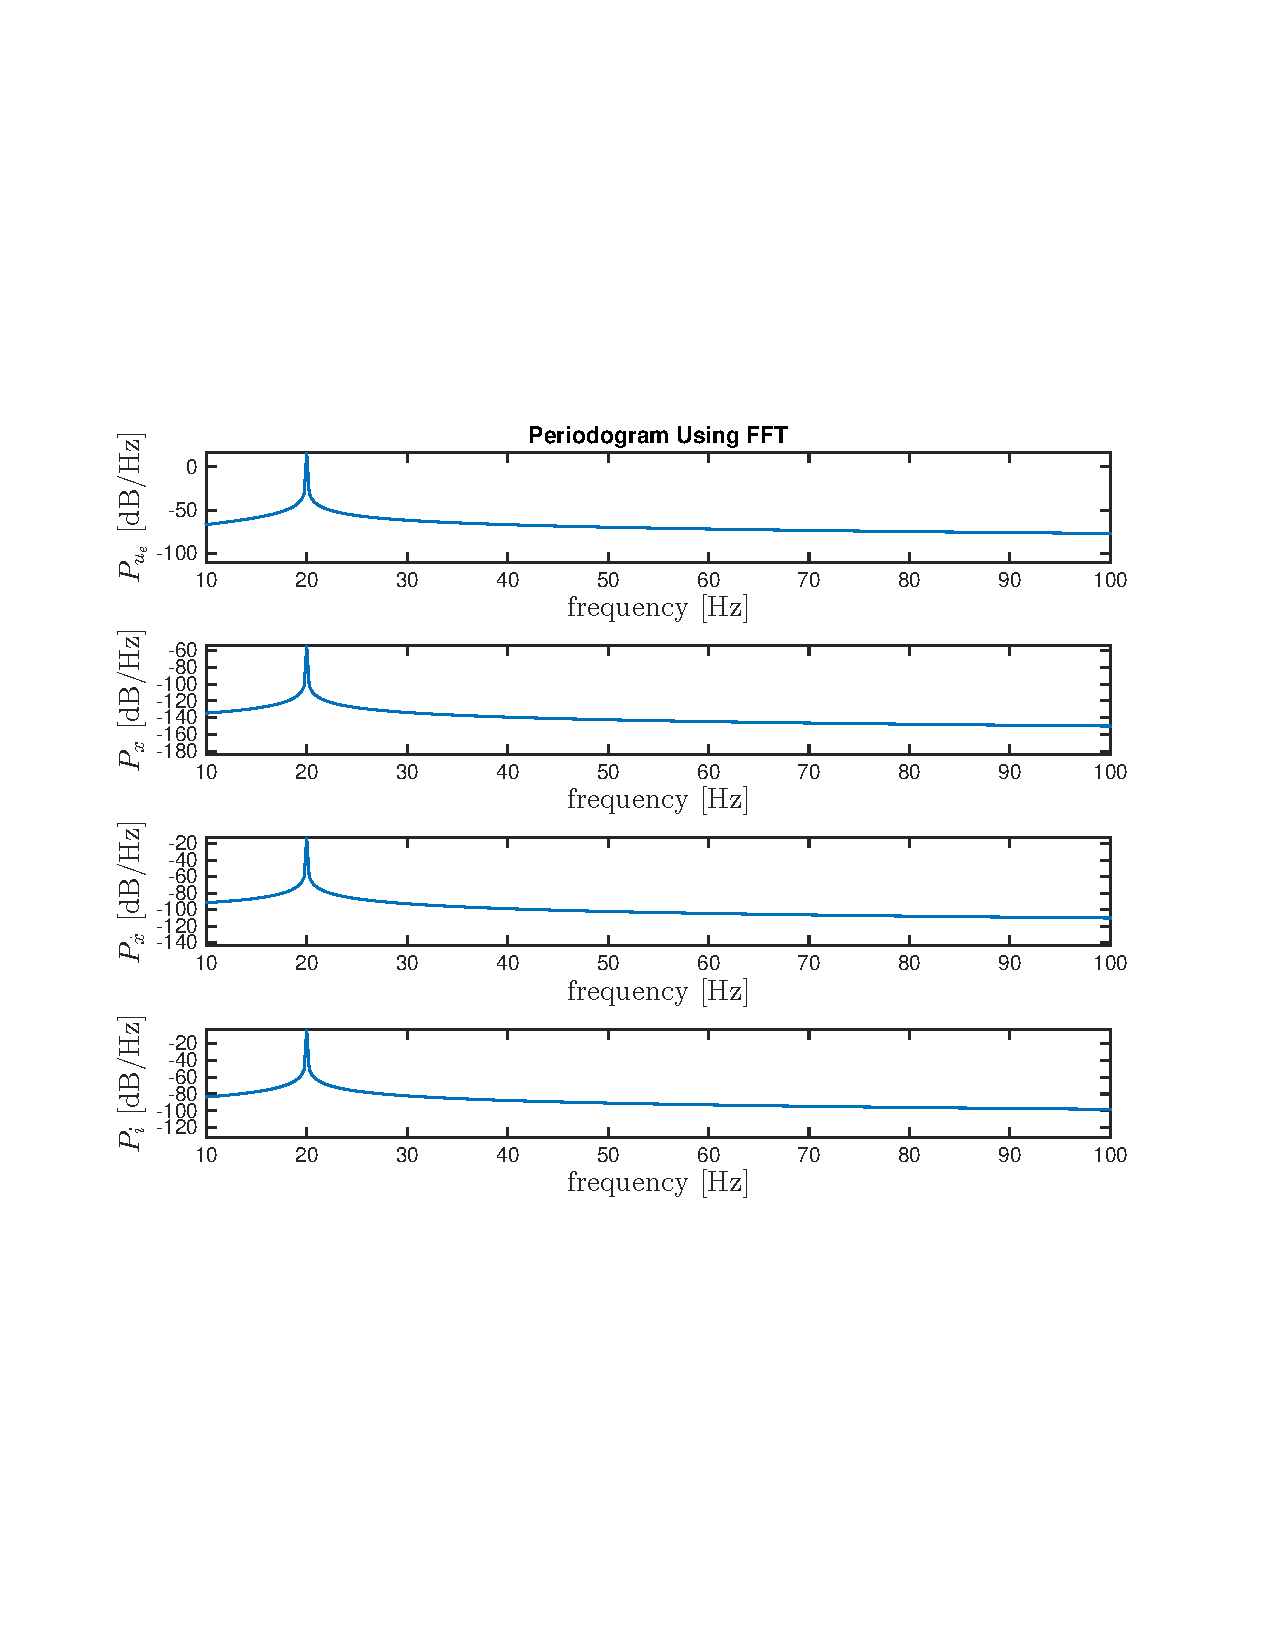
\includegraphics[trim=2cm 7cm 2cm 7cm, clip=true, totalheight=0.35\textheight, angle=0]{figures/p9freq.pdf}
\caption{PSD of $u_e$ and states}
\label{fig:responseLMf}
\end{figure}

First, comparing the response to the input $u_e$ from the nonlinear model with the linear model in the time domain (figure \ref{fig:NLMt}), the states response is almost exactly the same, but comparing the PSD of the states response (figure \ref{fig:NLMf} and figure \ref{fig:responseLMf}), we can see that the states response is not the same. Indeed, the linearised system is not affected by the harmonic distortion, there is only one frequency present in the states response, the one of 20$Hz$ (which has the same magnitude).
This result was expected because the nonlinear distortion only affects non-linear systems. Moreover, we have linearised the system with an input $u_e=0$ which means that we have a linearised system without harmonic, and then, we used a new input $u_e$ with a frequency $f_c=20Hz$, which means we only obtain a state response with an harmonic of a frequency of $f_c$.







\subsection{Harmonic distortion and fictitious disturbances}
In this section, we basically want to add a disturbance in order to obtain the same output with the linearised system than with the nonlinear system (the analysis is restrained to the second and third order harmonics). Thus, the output $i(t)$ should be
\begin{equation}
\label{eq:output}
y_{nl}(t)=A_1\sin(2\pi f_ct+\psi_1)+A_2\sin(4\pi f_ct+\psi_2)+A_3\sin(6\pi f_ct+\psi_3)
\end{equation}

\subsection*{Problem 10}
\addcontentsline{toc}{subsubsection}{Problem 10}
First, we extend our model with two input disturbances such that the linear output will also show the second and third order harmonics. The new linearised model is
\begin{align*}
   \dot{\text{x}} &= A\text{x} + B\text{u} +B_d\text{d}, \qquad with\ d = [d_{i1}, d_{i2}].\\
   y &= C\text{x}
\end{align*}



We know that $d_{i1} = A_{i1}\sin(4\pi f_ct)$ and $d_{i2} = A_{i2}\sin(6\pi f_ct)$ but we have to determine the magnitudes $A_{i1}$ and $A_{i2}$. As this disturbance can be considered as an input, we choose to take $B_d = [B\ B]$ and to find the right magnitudes to use.

In order to find $A_{i1}$ and $A_{i2}$, we evaluate the gain of the transfer function for the three different frequencies. Then, knowing the desired amplitude for each harmonic, we can find the magnitudes $A_{i1}$ and $A_{i2}$.

\begin{lstlisting}[language=Matlab]
sys=ss(A,B,C,[0]);
w = [2:2:6]*pi*fc;
[MAG,PHASE] = bode(sys,w)
MAG=[MAG(1) MAG(2) MAG(3)];
[Aifundamental, Ai1, Ai2] = Amplitude(3,1:3)./MAG % = 5.0212    0.0723    0.0792
\end{lstlisting}

\subsection*{Problem 11}
\addcontentsline{toc}{subsubsection}{Problem 11}
The disturbance is now added to our SIMULINK model (see figure \ref{fig:linearModelNoise}). The response to the input can be seen figure \ref{fig:responseNoiset} and the PSD figure \ref{fig:responseNoisef}.

\begin{figure}[H]
 \centering 
 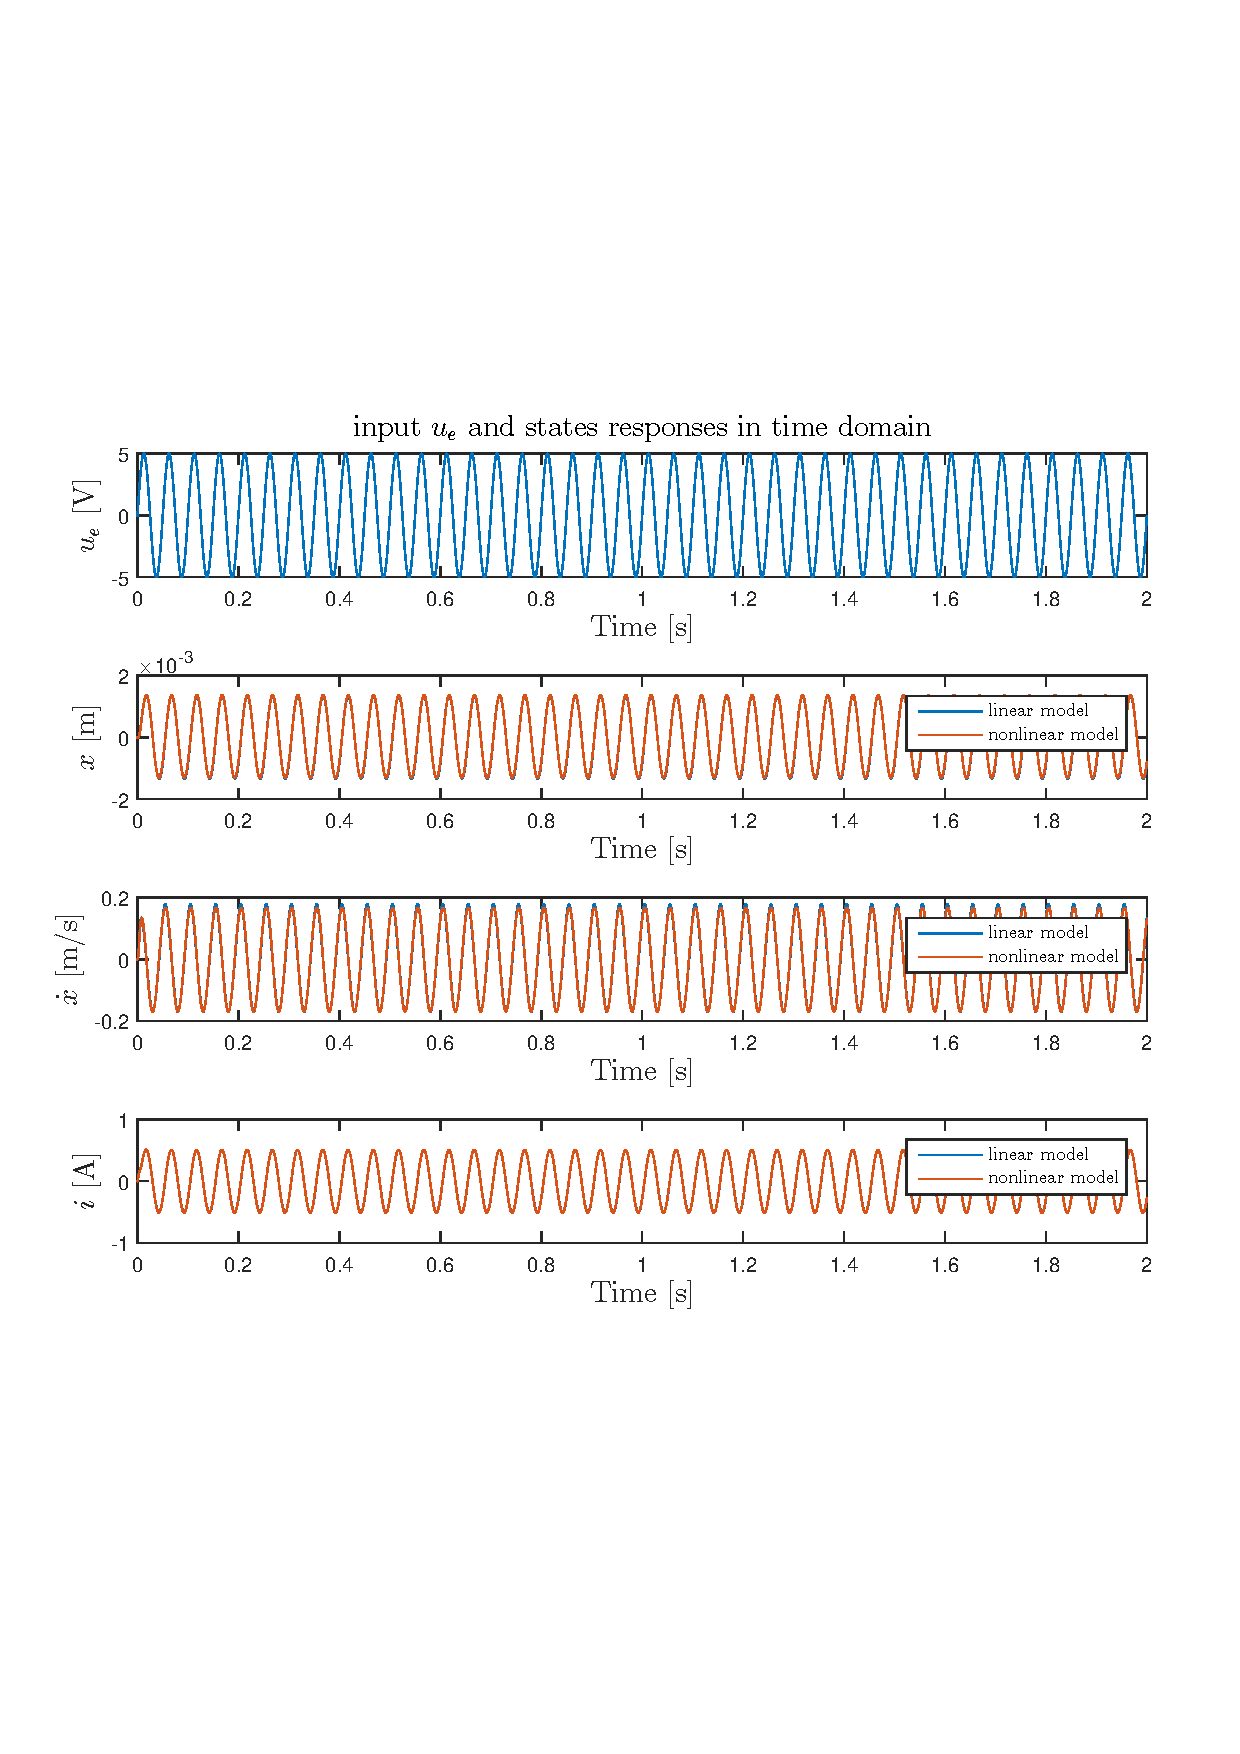
\includegraphics[trim=2cm 7cm 2cm 7cm, clip=true, totalheight=0.35\textheight, angle=0]{figures/p11time.pdf}
 \caption{response of the states to the input $u_e$ using the linearised model extended with disturbances and the nonlinear model}
 \label{fig:responseNoiset}
\end{figure}

\begin{figure}[H]
 \centering 
 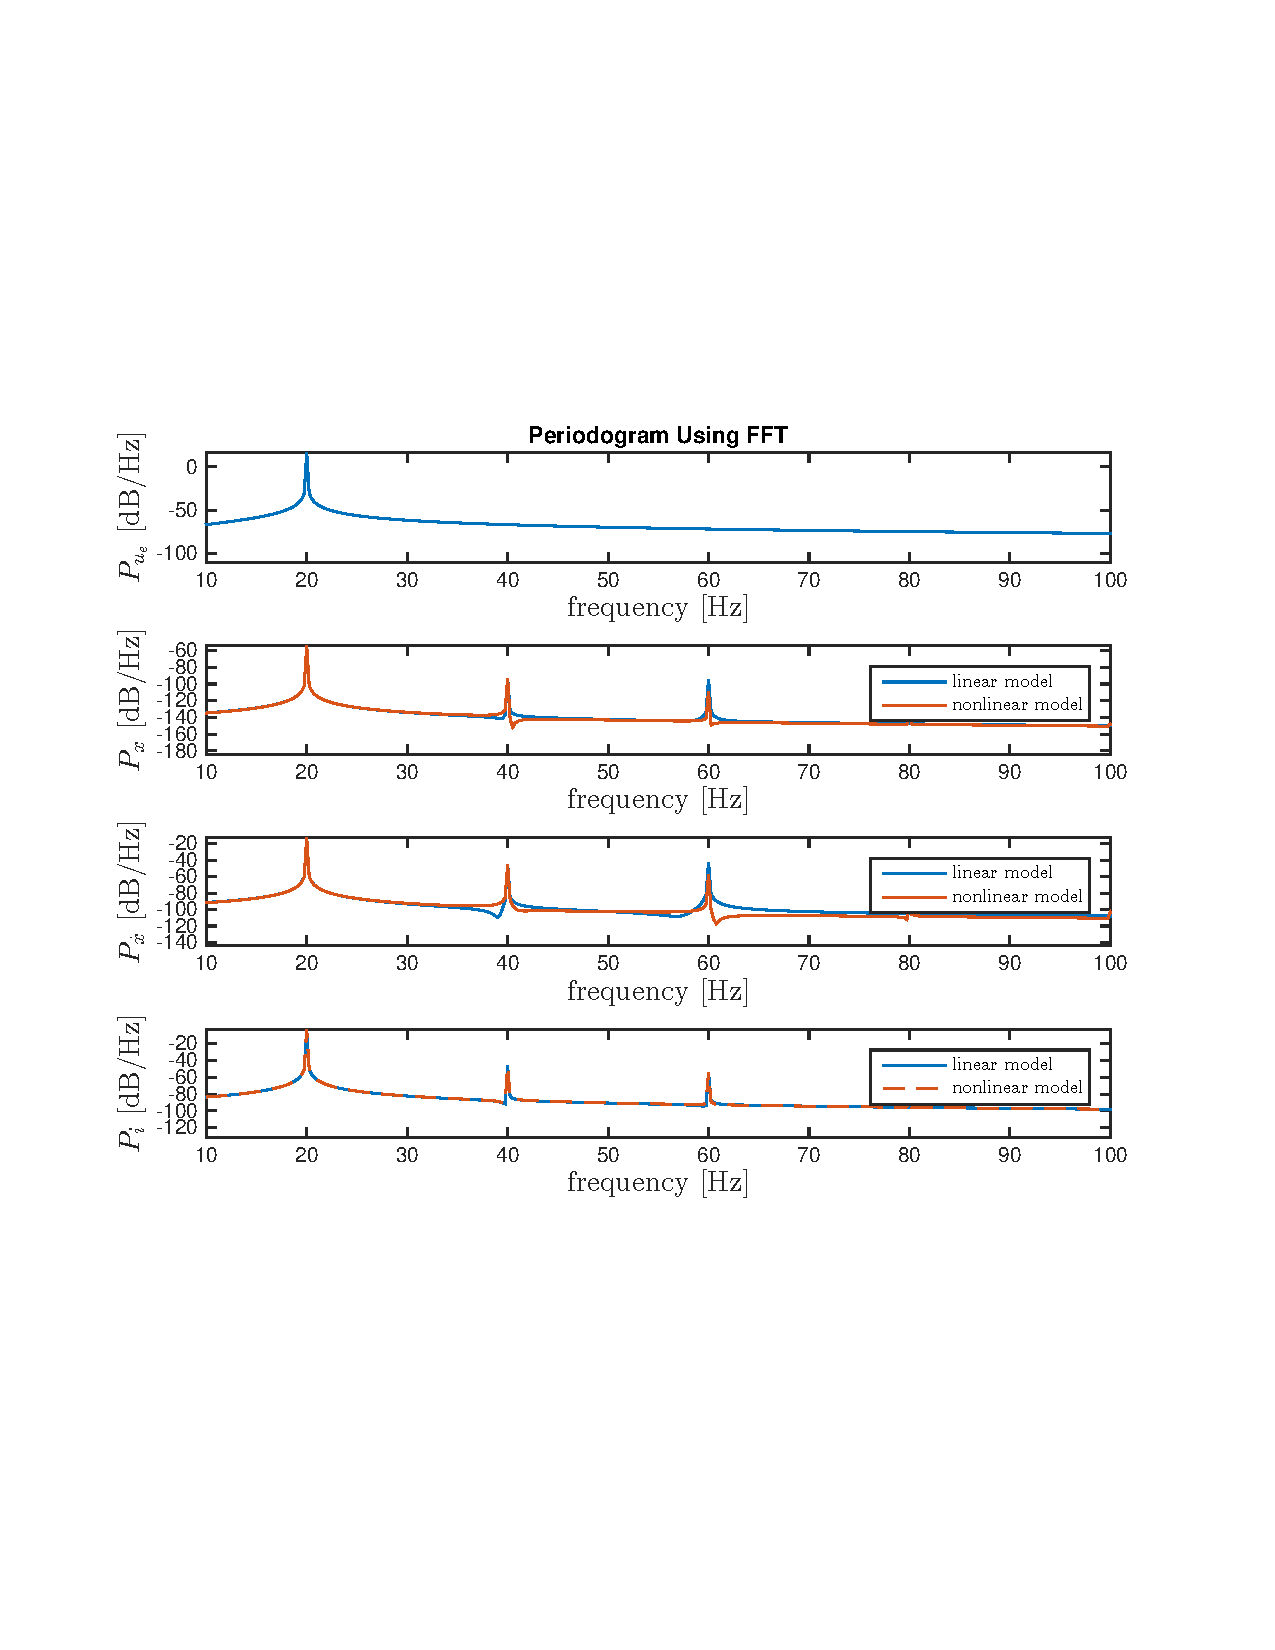
\includegraphics[trim=2cm 7cm 2cm 7cm, clip=true, totalheight=0.35\textheight, angle=0]{figures/p11freq.pdf}
 \caption{PSD of the states using the linearised model extended with disturbances and the nonlinear model}
 \label{fig:responseNoisef}
\end{figure}

We can see on both figures (\ref{fig:responseNoiset} and \ref{fig:responseNoisef}) that the responses are almost exactly the same (the plot of the response of the nonlinear model is over the one of the linear model). As expected, the two harmonic distortions of $40$ and $60$ $Hz$ are present with the right magnitude. The next distortions are of course missing. Also, the magnitude of the harmonics of state $i$ are almost perfect, but not the ones of the other states which is normal because the disturbance is designed for $i$.



\subsection{System discretization}
\subsection*{Problem 12}
\addcontentsline{toc}{subsubsection}{Problem 12}
We now want to discretize the continuous time linear model. As the smallest constant time is $\tau_2=0.0013\ s$, we will choose a sampling time $T_s=0.0001\ s$, that is to say 10 times faster. However, this sampling time is the $STEP\_SIZE$ of the simulation, so the sampling time should be different. Therefore, we will choose $T_s=0.0002\ s$.

Then, we can discretize the linear system using $c2d$ MATLAB function.

\begin{lstlisting}[language=Matlab]
Ts=0.0002; %[s]
[F,G]=c2d(A, B, Ts);
[F, Gd] = c2d(A, Bd, Ts);
lambdad=eig(F);
\end{lstlisting}

The eigenvalues, $\lambda_1=0.9426$, $\lambda_2=0.8869+0.0864i$ and $\lambda_3=0.8869-0.0864i$, of the discrete time system are inside the unit circle, which means that the system is still asymptotically stable. This result was expected because a discrete time system with a well chosen sampling time is supposed to have the same behavior and be the same system.


  \begin{thebibliography}{1}
	\bibitem{assign} Roberto Galeazzi, {\em Manual For Compulsory Exercise,}  2015.
  \end{thebibliography}

\end{document}
